We train on three targets of increasing dimension: GMM-40 ($d=2$), a 10-component Gaussian mixture in $d=16$, and the many-well MW-32 ($d=32$, $2^{16}$ modes).
We compare iDEM, AEM from scratch (\emph{cold}), explore$\to$anchor AEM (iDEM for 20 outer iterations, then anchored targets; the first phase is identical to the iDEM run with the same seed), and explore$\to$anchor AEM with replay proposals (AEM-R).
\Cref{tab:main} reports the final metrics and \cref{fig:curves} the training curves.

\paragraph{iDEM's fixed-point bias is visible, and AEM removes it.}
\Cref{cor:fixed} predicts that iDEM converges to the biased field $b_K$. On MW-32 this bias has a clear signature: the Gaussian coordinates of iDEM samples have variance $4.1\pm0.4$ instead of $1$, and the energy histogram is shifted ($\mathcal{E}$-$\mathcal{W}_1=44.5$). Every AEM variant brings the variance ratio to $1.04$--$1.05$ and lowers $\mathcal{E}$-$\mathcal{W}_1$ by $4$--$29\times$, with a better $\mathcal{W}_2$, at a 1\% higher energy budget.
On GMM-10 ($d=16$) the effect is the same but smaller: the within-mode variance ratio is $1.21$ for iDEM and $1.05$--$1.09$ for AEM, and $\mathcal{E}$-$\mathcal{W}_1$ falls from $1.57$ to $0.29$--$0.62$.
\Cref{fig:marginals} shows the effect directly: iDEM's Gaussian marginals are about twice too wide, its double-well marginals put mass between the wells, and its energy histogram is shifted by about $40$ units. The anchored model matches all three.
These quantities are governed by the within-mode posterior, where the anchor is informative.

\paragraph{In two dimensions there is nothing to fix.}
On GMM-40 all four methods perform similarly ($\mathcal{W}_2$ $4.6$--$5.0$, $\mathcal{E}$-$\mathcal{W}_1$ $0.71$--$0.92$, all 40 modes covered), and most differences are within one standard deviation. This matches the estimator study: in $d=2$, SNIS with $K=100$ is already nearly unbiased at the noise levels that matter. The within-mode variance ratio of $1.7$--$1.9$ is nearly the same for every method, so it reflects the sampler discretization ($\sigma_{\max}/\sigma_{\min}=7000$ with 500 steps) and not the regression target.


\begin{figure*}[t]
\centering
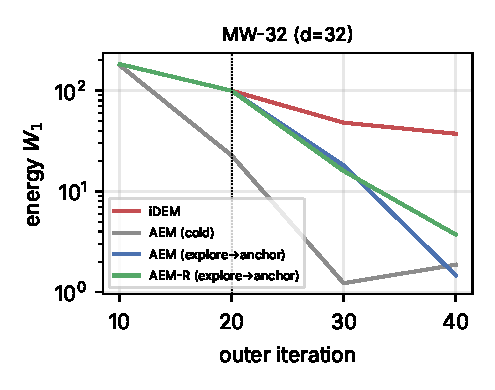
\includegraphics[width=\textwidth]{fig_curves.pdf}
\caption{\textbf{Energy $\mathcal{W}_1$ during training} (mean and min--max over 3 seeds). The dotted line marks the switch from exploration to anchoring in the explore$\to$anchor runs. Before it, those runs coincide with iDEM.}
\label{fig:curves}
\end{figure*}

\begin{figure}[t]
\centering
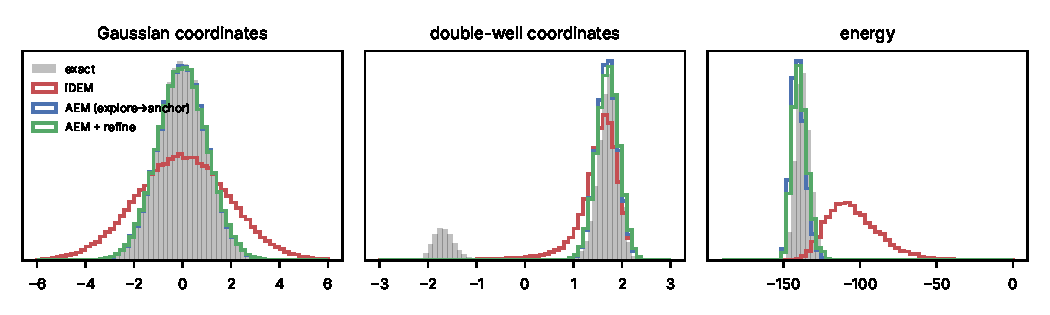
\includegraphics[width=\columnwidth]{fig_mw_marginals.pdf}
\caption{\textbf{MW-32 marginals} (samples pooled over 3 seeds) against exact samples (grey). iDEM's fixed-point bias widens the Gaussian coordinates, smears mass between the wells and shifts the energy distribution. AEM removes these distortions.}
\label{fig:marginals}
\end{figure}

\paragraph{Oracle buffer: testing the fixed point directly.}
To rule out explanations such as short training, the stability caps or the sampler loop, we remove the loop entirely. We train on a \emph{fixed buffer of $10^4$ exact samples} from $\pi$ (\texttt{oracle} mode; rows drawn without replacement), so the buffer law is exactly $\pi$ and \cref{cor:fixed} applies verbatim. We then measure the relative error of the learned score against the exact noised score $\nabla\log p_t$ at $x_t=x_0+\sigma_t\varepsilon$, $x_0\sim\pi$ (\cref{tab:oracle}).
On MW-32 the result is unambiguous. Trained on exact samples, iDEM learns a score whose relative error is $25.0\pm2.6$ at $\sigma_t=1$ and $35.0\pm2.3$ at $\sigma_t=2$ (3 seeds), against $0.140\pm0.003$ and $0.074\pm0.004$ for AEM. Ten times more proposals barely help iDEM: with $K=1000$ (one seed) its error is still $9.8$--$27.6$. This is what one expects from an SNIS bias that decays like $1/K$ with a constant that is exponential in $d$. With a perfect buffer, AEM also gets the mode weights right: in seed 0 the fraction of double-well coordinates in the major well is $0.837$, against a true $0.844$ (iDEM: $0.898$). So the mode-weight deficits of \cref{tab:main} come from the self-generated buffer, as \cref{thm:contraction} predicts, and not from the anchored target.
On GMM-10, where the TSI/DSI combination is exact within each unit-variance component, the two methods learn similar scores at $\sigma_t\ge0.3$ (differences within one standard deviation); AEM is more accurate at $\sigma_t\le0.1$ in the mean.
On the molecular targets we rank the models by held-out denoising loss, which by \cref{prop:diag}(ii) differs between two models by exactly the difference of their score errors (normalized as $\tilde L=\sigma_t^2L/d_{\mathrm{eff}}$; the held-out configurations are disjoint from every seed's buffer). On DW-4 the AEM model has the lower score error at every noise level and in every seed at $\sigma_t\ge0.3$, by a margin that grows from $0.02$ to $10.9$ (\cref{tab:diag}); its samples also have a lower interatomic-distance $\mathcal{W}_1$ in every seed ($0.035$--$0.101$ vs.\ $0.085$--$0.250$). On LJ-13, AEM is better at $\sigma_t\in\{1,2\}$ in all seeds, but slightly worse in the mean at $\sigma_t\le0.3$ (not consistent across seeds), and the gaps are small compared with DW-4. The oracle-trained LJ-13 models of both methods produce some very high-energy samples, so we do not use their sample metrics.

